\documentclass[conference]{IEEEtran}
\IEEEoverridecommandlockouts
\usepackage{cite}
\usepackage{amsmath,amssymb}
\usepackage{graphicx}
\usepackage{booktabs}
\usepackage{tabularx}
\usepackage{multirow}
\usepackage{url}
\usepackage{microtype}
\graphicspath{{figures/}}

\begin{document}
\title{Multi-Agent Debate Framework using Evidence Disagreement Triggering and Conflict-Type Classification}

\author{
\IEEEauthorblockN{M.~Marimuthu}
\IEEEauthorblockA{\textit{Faculty, School of Computer Science and Engineering (SCOPE)}\\
\textit{VIT Chennai, India}}
\vspace{0.8em}
\IEEEauthorblockN{M.~Reddy Sasi Kiran \hspace{1em} Suhas Koheda \hspace{1em} C.~R.~Suhas}
\IEEEauthorblockA{\textit{School of Computer Science and Engineering (SCOPE)}\\
\textit{VIT Chennai, India}}
}
\maketitle

\begin{abstract}
We built Evidence-MAD to answer a practical question: should a system debate every answer, or wait until its sources disagree? The system retrieves material from several sources, turns it into short claims, and uses a natural-language-inference model to decide whether the claims agree, conflict, or remain uncertain. When the recorded state is disagreement, a conflict classifier selects a strategy for a debate. We inspected the six system folders in the project results and kept the 96 questions that have a trace in every folder. The traces show that Evidence-MAD triggered debate on 22 of 96 questions (22.9\%), while the Standard MAD configuration triggered on 50 (52.1\%). The median recorded latency was 50.0 seconds for Evidence-MAD and 55.0 seconds for Standard MAD. These are observations from one live run, not evidence that the proposed system answers more questions correctly: the matched traces have no gold answer labels, and key-fact accuracy was not scored. The recorded model identifiers also vary across traces and systems. We present the plots as a description of system behavior and treat answer quality and causal comparisons as open evaluation questions.
\end{abstract}

\begin{IEEEkeywords}
large language models, multi-agent systems, retrieval-augmented generation, natural language inference, debate, evidence verification
\end{IEEEkeywords}

\section{Introduction}
A search system can return several answers to the same question. Sometimes the sources agree. Sometimes they use different dates, versions, populations, or meanings. A multi-agent debate can be useful when those answers disagree, but debate also adds model calls and waiting time. Retrieval-augmented generation connects a language model to external information at answer time \cite{lewis2020rag}. Multi-agent debate lets language-model agents critique and revise candidate answers \cite{du2024icml}. Evidence-MAD puts an evidence check between retrieval and debate.

The system has two main choices. First, it uses a gate to decide whether the available claims show disagreement. Second, when the gate opens, it assigns a conflict type and selects a matching prompt strategy. The implemented types are factual, temporal, version, contextual, and source-related. The idea is straightforward: different disagreements may need different questions from a critic. A date conflict calls for aligning dates; a version conflict calls for naming the release; and a contextual conflict calls for checking population or conditions.

This paper reports what is present in the current result traces. The original question file contains 100 questions. We selected the intersection of the six result folders, which contains 96 question IDs. Each of the six systems has one saved trace for each of those IDs. Four questions without traces shared by all six systems are excluded from these plots. We do not score answers because the matched trace bundle does not contain the gold labels needed to do that correctly.

The main finding is about routing, not answer quality. Evidence-MAD recorded debate on 22 questions, compared with 50 for Standard MAD. This shows a lower observed debate rate for the proposed configuration in this run. It does not show that the gate kept the right cases out of debate. The results also show long latency tails, failed internal model calls, many insufficient-evidence states, and a mixture of model identifiers across systems. Those details matter when reading the comparison.

This paper makes three limited contributions. It describes the implemented retrieval, gate, and debate path; gives trace-derived counts and plots for six configurations on the same 96 questions; and records limits that prevent an answer-quality or causal claim. The paper is intended as a transparent report of a prototype run. It is not a benchmark result establishing that Evidence-MAD is better than the alternatives.

\section{Related Work}
The literature review in the project presentation groups prior work into debate protocols, selective debate, and evidence conflict handling. We include all 16 papers listed there. This is a focused project review, not a systematic review of every multi-agent or retrieval system.

\subsection{Multi-agent debate}
ReConcile uses a round-table discussion with diverse language models and confidence-weighted voting \cite{chen2024reconcile}. Du et al. study repeated proposal, critique, and revision to improve reasoning and factuality \cite{du2024icml}. DoT uses a tit-for-tat discussion and a judge that can stop the process when further discussion is not useful \cite{liang2024dot}. ChatEval applies role-diverse debate to evaluating generated text rather than answering evidence conflicts \cite{chan2024chateval}. Khan et al. study two stronger agents arguing opposite answers for a weaker judge, and FORD compares debate structures to study whether different language models can reach consistent decisions \cite{khan2024persuasive,xiong2023ford}.

These papers establish that agent roles, debate structure, and stopping rules are important design choices. They do not, by themselves, show that debate should start only after a contradiction between independently retrieved claims. Our system makes that pre-debate decision explicit. At the same time, the current experiment does not establish that its decision improves answer quality.

\subsection{Selective debate and adaptive collaboration}
DOWN starts debate according to the confidence of an initial answer \cite{eo2025down}. B\k{a}ba and Chudziak also use confidence gating, in their case for argument-relation classification \cite{baba2026confidence}. These works are close to Evidence-MAD because both ask whether every case needs a debate. Their trigger is model confidence on the task, while the Evidence-MAD gate is intended to use relations among retrieved claims. Choi et al. separate the contributions of voting and debate and caution that debate should be evaluated against simpler aggregation strategies \cite{choi2025debate}. That result supports our choice to treat debate cost and answer quality as separate measurements.

\subsection{Retrieval and conflicting evidence}
MADKE adds a shared retrieval knowledge pool to a multi-agent debate and lets agents select knowledge during discussion \cite{wang2025madke}. MAIN-RAG uses agents to filter and score retrieved documents before generation \cite{chang2025mainrag}. MADAM-RAG directly studies retrieval with conflicting evidence and uses agents to discuss ambiguity, misinformation, and noise \cite{wang2025madamrag}. Tool-MAD assigns different tools to agents and can adapt retrieval as the debate develops \cite{jeong2026toolmad}. These systems show that retrieval and debate have already been combined in several ways. Evidence-MAD's design question is narrower: whether a comparison of claims should open the debate path before conflict resolution begins.

Other work focuses directly on conflict identification and response. DRAGged into Conflicts introduces a taxonomy for conflicts among search results and studies response behavior in a search-augmented single-model setting \cite{cattan2025dragged}. Xu et al. survey knowledge conflicts, including disagreement between context and model memory, between context sources, and within model knowledge \cite{xu2024conflict}. SMADE-IE uses sparse, evidence-driven debate for zero-shot information extraction, where agents may disagree over labels or extracted structures \cite{huang2026smade}. These works make it clear that neither evidence conflict nor evidence-informed debate is new on its own.

\subsection{Positioning of this study}
The system tested here combines three implemented steps: normalize claims from separate retrieval agents, use pairwise NLI plus query-aware rules to assign an evidence state, and, on disagreement, classify the conflict and select a type-specific debate prompt. It differs from confidence-only gating by using retrieved claim relations as the intended trigger. It differs from document filtering by making the conflict state control whether the debate stage runs. It differs from conflict taxonomies that guide a single answer by passing the type into a multi-agent resolution prompt. These are distinctions in system design, not proof of priority or novelty over every related method. The study is an implementation and a first trace-based comparison; its current data do not demonstrate that the combined design is more accurate or more useful than the cited systems.

\section{System Design}
Figure~\ref{fig:architecture} summarizes the implemented control flow and its three response paths.
\begin{figure*}[t]
\centering
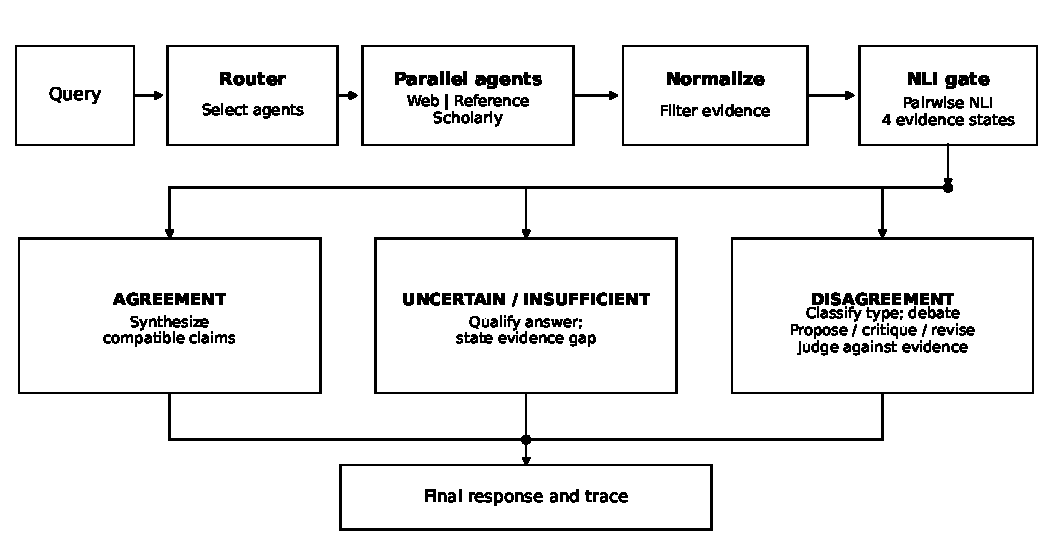
\includegraphics[width=0.96\textwidth]{evidence_mad_architecture.pdf}
\caption{Implemented Evidence-MAD control flow. The four-state evidence gate sends disagreement to conflict classification and typed debate. Agreement, uncertain, and insufficient states follow separate answer paths. Only the disagreement path enters conflict classification and typed debate.}
\label{fig:architecture}
\end{figure*}
\subsection{Retrieval and claim preparation}
For each query, the system routes work to retrieval agents and collects the returned evidence. The saved run signature lists DuckDuckGo, Wikipedia, Wikidata, Crossref, OpenAlex, arXiv, and Europe PMC as configured sources. Retrieved snippets are passed through a normalizer that produces short claims and retains source information. A relevance filter can remove results that do not appear connected to the question. The \textsc{No Relevance Filter} configuration disables that filtering step.

The normalization stage is important because later decisions use the claims it produces, not the full original pages. If the normalizer leaves out a date, scope, or qualification, the gate cannot recover it. Each trace records the claims, source metadata, evidence state, debate activity, final answer, and per-query metrics. This makes it possible to inspect why the system took a particular path, even when the final answer cannot be scored.

\subsection{Evidence gate}
The gate compares available claim pairs in both directions with an NLI model. NLI models estimate whether one sentence entails, contradicts, or is neutral toward another; MNLI is a standard broad-coverage resource for this task \cite{williams2018mnli}. The trace metadata identifies the Transformers checkpoint as \texttt{ynie/roberta-large-snli\_mnli\_fever\_anli\_R1\_R2\_R3-nli}. The implementation combines pairwise inference output with query-aware logic and assigns an evidence state: \textsc{agreement}, \textsc{disagreement}, \textsc{uncertain}, or \textsc{insufficient}. In the proposed configuration, disagreement is the state that routes the trace to conflict classification and debate. Uncertain and insufficient states do not count as affirmative evidence of agreement.

This rule makes the gate simple to inspect. It also creates a risk: a real conflict that is assigned uncertain or insufficient will not reach the debate stage. That is why debate rate alone is not enough to evaluate the gate. A proper test needs independently labelled evidence conflicts and answers, neither of which is available for the 96 matched traces.

\subsection{Conflict-aware debate}
When the proposed system detects disagreement, a classifier selects a prompt strategy from factual, temporal, version, contextual, and source-related types. The debate uses proposer, critic, reviser, and judge roles. A debate can stop after a critic finds no unresolved objection, when the round limit is reached, or when a stage fails. The trace records the debate rounds and stop reason when available.

The six configurations differ in their intended settings. \textsc{Single LLM} produces a direct answer without retrieval-based debate. \textsc{Standard MAD} uses a generic debate strategy and is configured to debate when there is usable evidence. \textsc{Proposed MAD} uses the evidence gate and typed strategies. The three ablations are named \textsc{No Gate}, \textsc{No Typed Strategy}, and \textsc{No Relevance Filter}. These names describe the intended configuration changes; the saved values in the trace are used for all reported counts. The observed triggers do not always match the idealized configuration description, so we report the outcomes recorded in traces rather than assuming every requested stage completed.

\subsection{Trace interpretation}
A trace with \texttt{evaluation\_status=success} means that the evaluator wrote a completed record. It does not mean that every internal model call succeeded or that the answer is correct. For example, traces can contain a final answer after a proposer call failed. We distinguish completed records from successful internal calls in the results and do not treat trace completion as answer accuracy.

\section{Experimental Method}
\subsection{Matched question set}
The source dataset has 100 question IDs. We used the 96 IDs that appear in every one of the six system folders. This gives a matched set for descriptive comparisons of routing, latency, and call counts. Traces for questions outside this intersection remain in the original results archive and are not included in this analysis folder. Each included system folder contains 96 trace files, for 576 trace records in total.

The questions cover everyday factual prompts and specialized topics, as shown by the trace queries. The current analysis does not claim that the set is random or representative of search use. More importantly, the copied traces do not contain a usable gold answer label for each question. The saved metrics show zero key-fact samples scored. We therefore do not calculate accuracy, precision, recall, F1, missed-conflict rate, or unnecessary-debate rate. Assigning these values from system outputs would confuse a model's own decisions with ground truth.

\subsection{Configurations and recorded model metadata}
The trace signatures use more than one OpenCode model identifier. Table~\ref{tab:modelmix} gives the counts recorded in each system folder. The values show that the comparison is not model-uniform. The signatures name \texttt{console-openrouter/cohere/north-mini-code:free} and \texttt{console-openrouter/openrouter/free}; they do not independently verify the provider that served each response. We keep the recorded identifiers as metadata and do not infer model behavior from the alias names.

\begin{table}[t]
\centering
\caption{OpenCode model identifiers recorded in each system's 96 traces.}
\label{tab:modelmix}
\scriptsize
\begin{tabular}{lrr}
\toprule
System & Cohere alias & OpenRouter free alias\\
\midrule
Single LLM & 32 & 64\\
Standard MAD & 88 & 8\\
Evidence-MAD & 91 & 5\\
No Gate & 86 & 10\\
No Typed Strategy & 92 & 4\\
No Relevance Filter & 91 & 5\\
\bottomrule
\end{tabular}
\end{table}

The run signature also records \texttt{llama-3.3-70b-versatile} as the general LLM setting and the NLI checkpoint described above. The same signature lists the source providers in Section III-A. Because the model identifier mixture differs by system, the timing and routing results are descriptive observations from the saved run, not a controlled comparison that isolates only the system design.

\subsection{Measures}
We calculate debate activation as the fraction of traces where the saved \texttt{debate\_triggered} field is true. Latency uses the per-trace \texttt{metrics.latency\_seconds} field. The median and empirical 95th percentile summarize the distribution. Successful and failed call averages use \texttt{total\_llm\_calls\_ok} and \texttt{total\_llm\_calls\_failed}. Evidence-state counts come from the trace metric field, and retrieval coverage uses the recorded usable-agent and claim counts.

These are operational measures. They do not establish whether a debate was necessary, whether a conflict was missed, or whether the final response was correct. Those questions need labels created independently of the system outputs. We report no significance tests because the result is a single run with a small matched set and non-uniform model metadata.

\subsection{Reproducibility}
The analysis folder contains copies of the matched traces, a JSON summary recalculated from those traces, and the plotting script. The source run was live, so web results and network timings may change on a repeat. The plots are generated with Matplotlib using white backgrounds and black text. The analysis can be reproduced by running \texttt{python analysis/generate\_plots.py} from the analysis folder in the project environment; the script reads the original results path recorded in the file.

\section{Results}
\subsection{Debate activation}
Evidence-MAD recorded debate on 22 of 96 questions (22.9\%). Standard MAD recorded debate on 50 (52.1\%). The \textsc{No Gate} configuration also recorded 50 triggers. \textsc{No Typed Strategy} recorded 23 (24.0\%), and \textsc{No Relevance Filter} recorded 18 (18.8\%). The single-LLM baseline recorded no debate. Figure~\ref{fig:debate} shows these values.

These counts show that the proposed configuration debated less often than Standard MAD in this run. They do not tell us whether the 74 questions without an Evidence-MAD debate were appropriate cases to skip. Because the traces lack conflict labels, we cannot separate correct avoided debates from missed conflicts. The difference is a useful routing observation and a clear target for a labelled follow-up evaluation.

\begin{figure}[t]
\centering
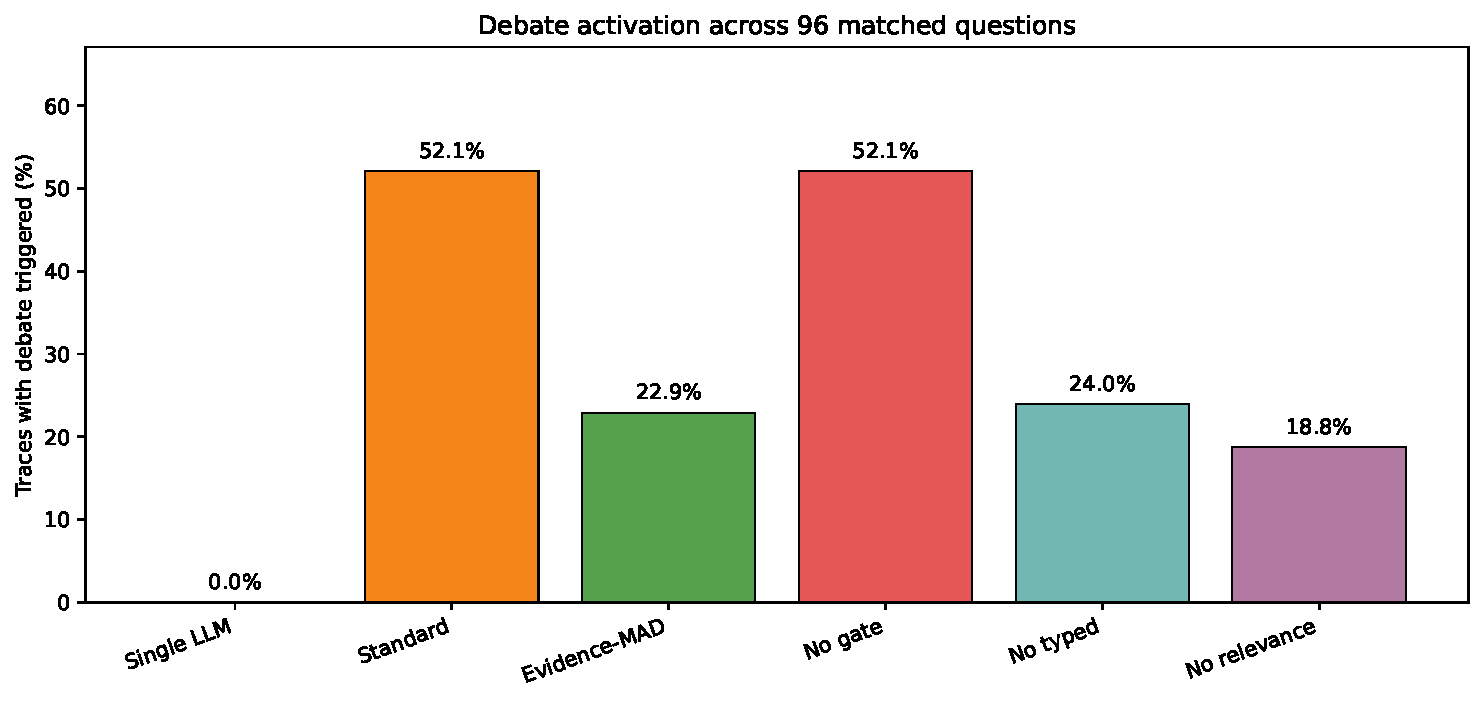
\includegraphics[width=\columnwidth]{debate_activation.pdf}
\caption{Fraction of matched traces with debate recorded as triggered. The Single LLM system has no debate stage.}
\label{fig:debate}
\end{figure}

\subsection{Whether a triggered debate completed}
A debate trigger does not mean a debate finished. In the Evidence-MAD traces, 16 of the 22 triggered debates were recorded as completed, five failed, and one was partial. Standard MAD recorded 29 completed and 21 failed outcomes among its 50 triggered debates. The no-gate configuration recorded 28 completed, 21 failed, and one partial outcome. These counts come from the debate outcome object, because the separate metrics field does not carry a status for every trace. Figure~\ref{fig:outcomes} includes both triggered outcomes and questions where debate was not triggered. The failure counts make clear that a lower debate count also changes the number of opportunities for a debate stage to fail. A useful future comparison should report answer quality and completed-debate rate together.

\begin{figure}[t]
\centering
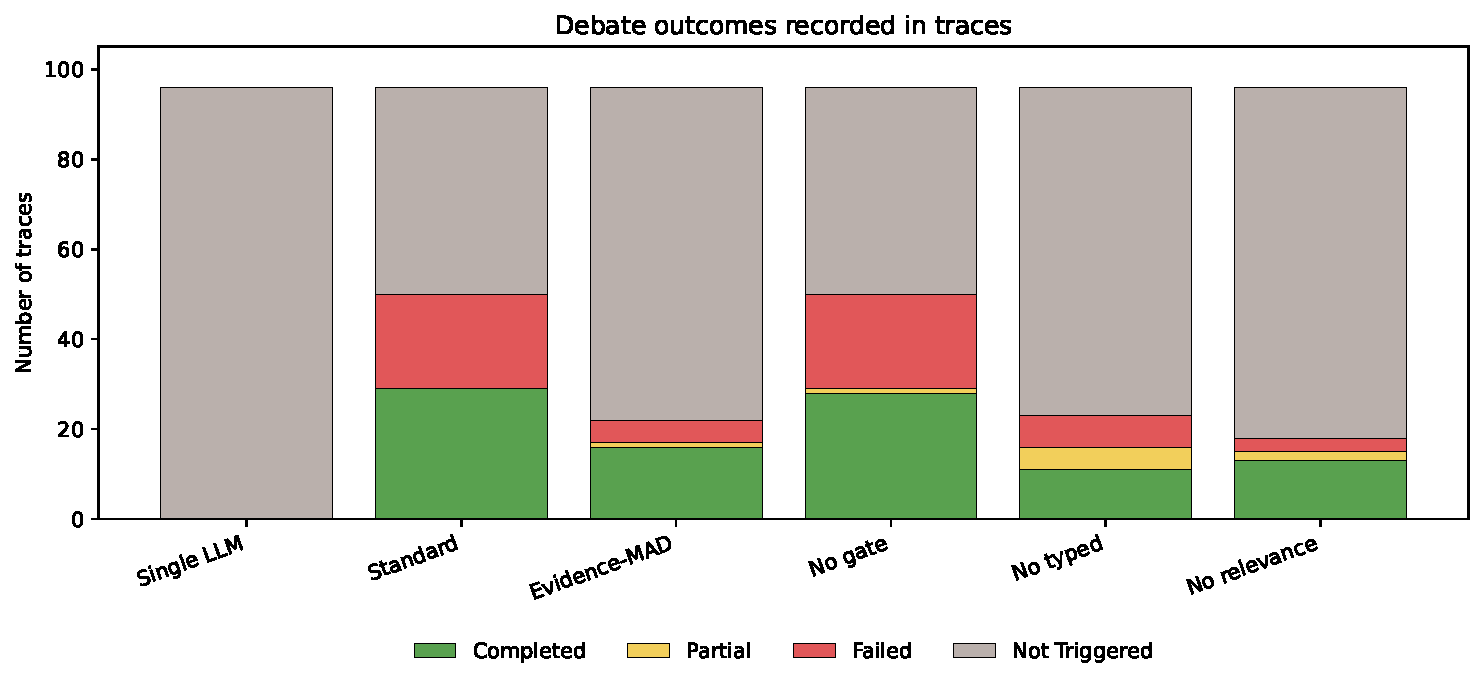
\includegraphics[width=\columnwidth]{debate_outcomes.pdf}
\caption{Recorded debate outcomes. The completed, partial, and failed segments apply to traces with a debate trigger; the remaining segment had no trigger.}
\label{fig:outcomes}
\end{figure}

\subsection{Evidence states}
For Evidence-MAD, the trace states were insufficient in 47 cases, uncertain in 26, disagreement in 22, and agreement in one. Only the 22 disagreement traces triggered debate. Standard MAD's traces recorded 46 insufficient states, 29 uncertain states, 16 disagreement states, and five agreement states, while debate was triggered in 50 traces. This gap reflects the way the baseline can force a debate when usable evidence exists; it should not be interpreted as 50 independently verified conflicts. Figure~\ref{fig:states} gives counts for all systems.

The high number of insufficient and uncertain states is a practical limitation. In 73 of the 96 Evidence-MAD traces, the recorded state was not disagreement. Some of these questions may genuinely lack comparable evidence; others may reflect retrieval or normalization problems. The traces alone do not tell us which explanation applies. A future evaluation should label the retrieved claim pairs and record whether each state is appropriate.

\begin{figure}[t]
\centering
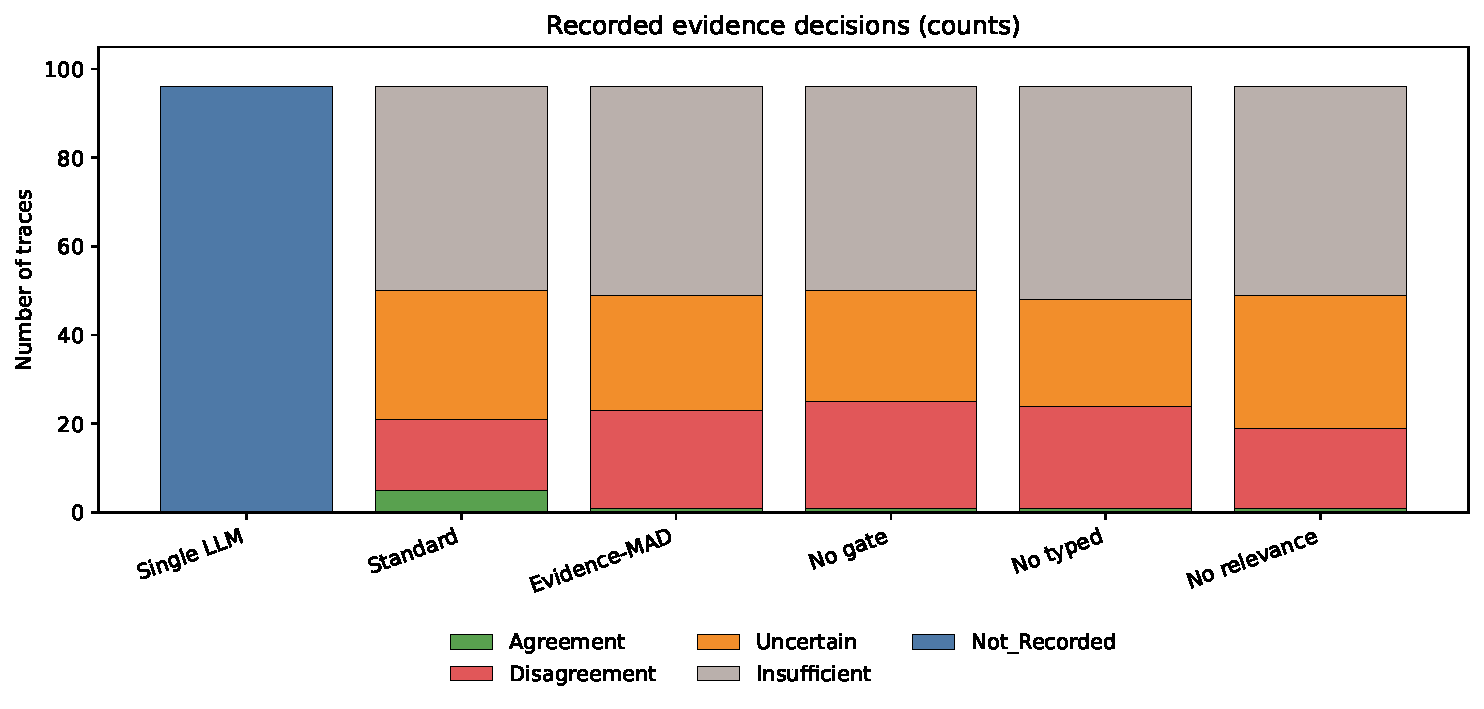
\includegraphics[width=\columnwidth]{evidence_states.pdf}
\caption{Evidence-state counts from each system's traces. Single LLM does not record an evidence state.}
\label{fig:states}
\end{figure}

\subsection{Latency and model calls}
Evidence-MAD had a median latency of 50.0 seconds and a 95th percentile of 232.7 seconds. Standard MAD had a median of 55.0 seconds and a 95th percentile of 211.5 seconds. The medians are close, while the proposed system has a longer observed upper tail. The single-LLM baseline was faster in this run, with a 16.8-second median and a 26.5-second 95th percentile. Figure~\ref{fig:latency} uses a logarithmic axis to show both typical and long-tail latency.

Evidence-MAD averaged 1.85 successful and 0.39 failed model calls per question. Standard MAD averaged 1.42 successful and 0.49 failed calls. The no-typed-strategy ablation averaged 1.90 successful and 0.49 failed calls, the highest successful-call mean among the retrieval systems. These averages include calls outside the debate roles, such as normalization. They should not be read as a debate-only cost. Figure~\ref{fig:calls} displays the saved call counts.

\begin{figure}[t]
\centering
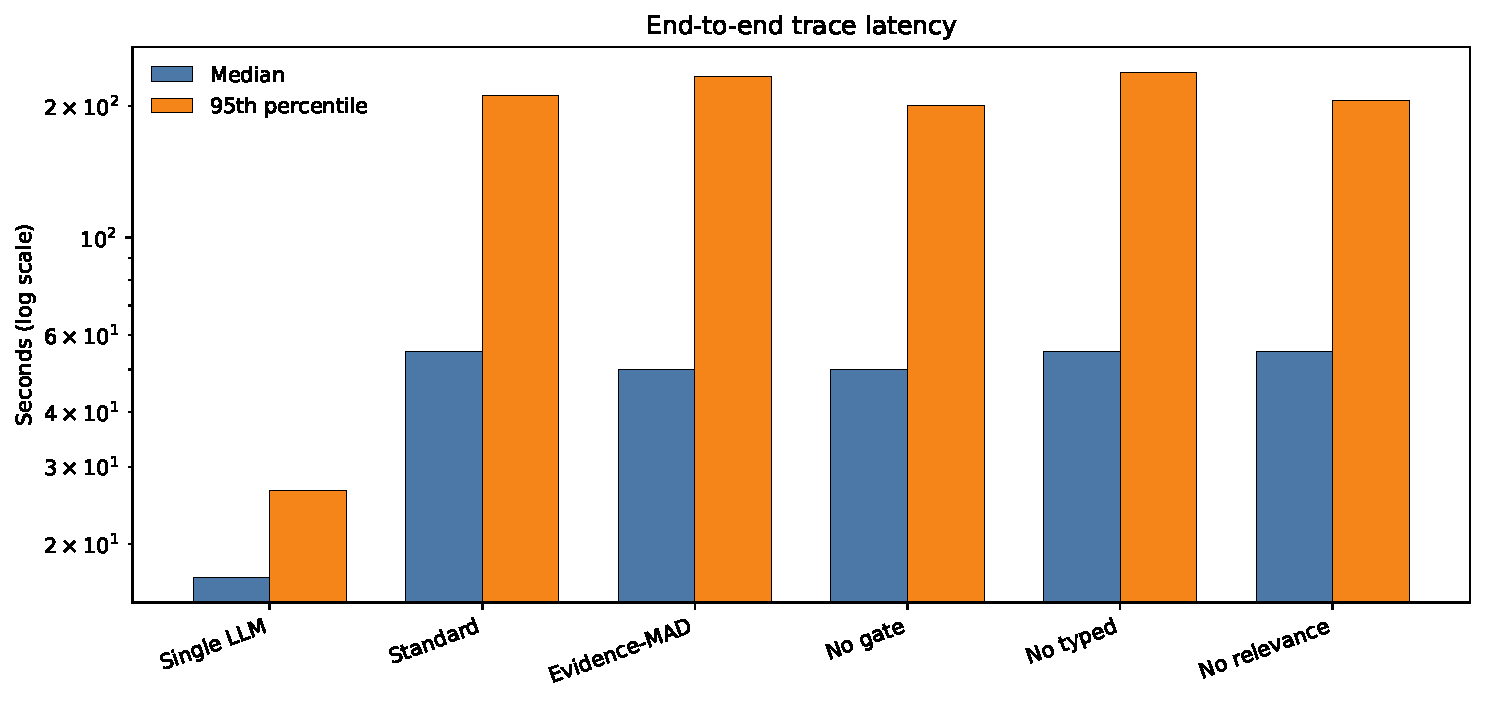
\includegraphics[width=\columnwidth]{latency.pdf}
\caption{Median and 95th-percentile latency for the matched traces. The vertical axis is logarithmic.}
\label{fig:latency}
\end{figure}

\begin{figure}[t]
\centering
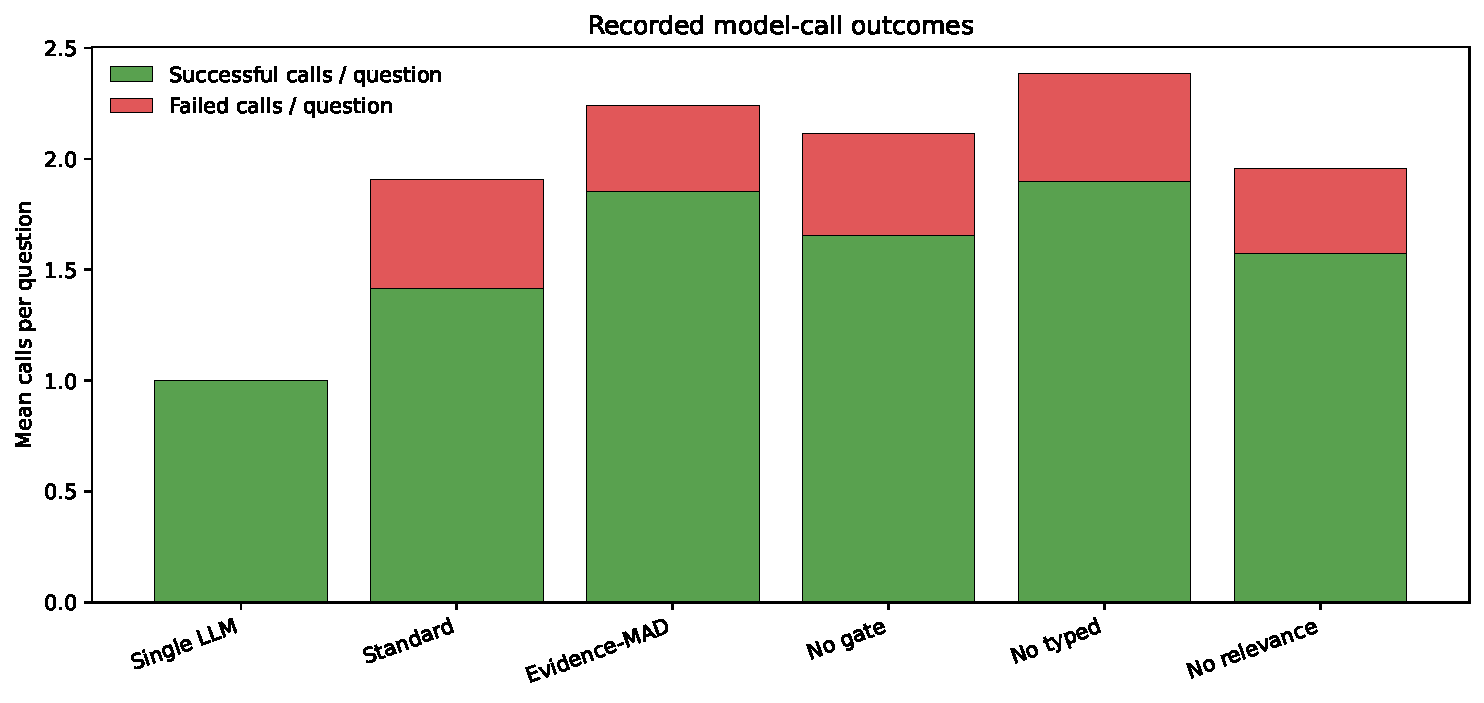
\includegraphics[width=\columnwidth]{model_calls.pdf}
\caption{Mean successful and failed model calls per question, as recorded in each trace.}
\label{fig:calls}
\end{figure}

\subsection{Retrieval output and model metadata}
The retrieval systems recorded about 1.24--1.31 usable agents per question on average. Evidence-MAD recorded 1.31, and Standard MAD recorded 1.24. This mean is low relative to the configured set of retrieval sources. It indicates that many traces had only a small amount of usable evidence available to the next stage. The call to source count is not one-to-one: an agent may use multiple sources, and a source may produce several snippets. Figure~\ref{fig:retrieval} shows usable agents and claims recorded in the traces.

Figure~\ref{fig:modelmix} shows the model identifiers in the trace signatures. The single-LLM folder contains 64 traces with the OpenRouter free alias and 32 with the Cohere alias. The other systems are mostly Cohere-alias traces, with between four and ten OpenRouter-alias traces each. This imbalance is large enough that it limits direct system-to-system interpretation. These labels come from the saved signature and are not an independent audit of the API route used at call time.

\begin{figure}[t]
\centering
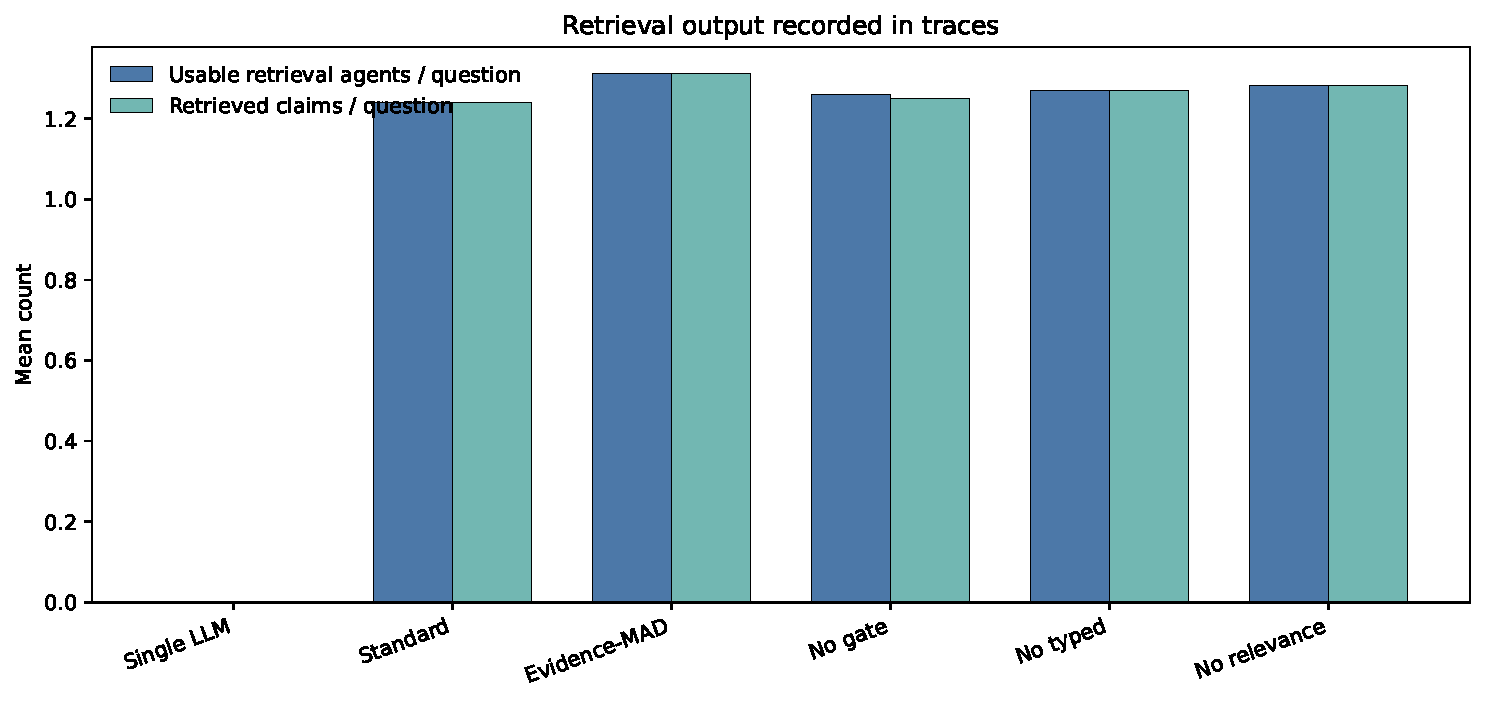
\includegraphics[width=\columnwidth]{retrieval_coverage.pdf}
\caption{Mean usable retrieval agents and extracted claims per question.}
\label{fig:retrieval}
\end{figure}

\begin{figure}[t]
\centering
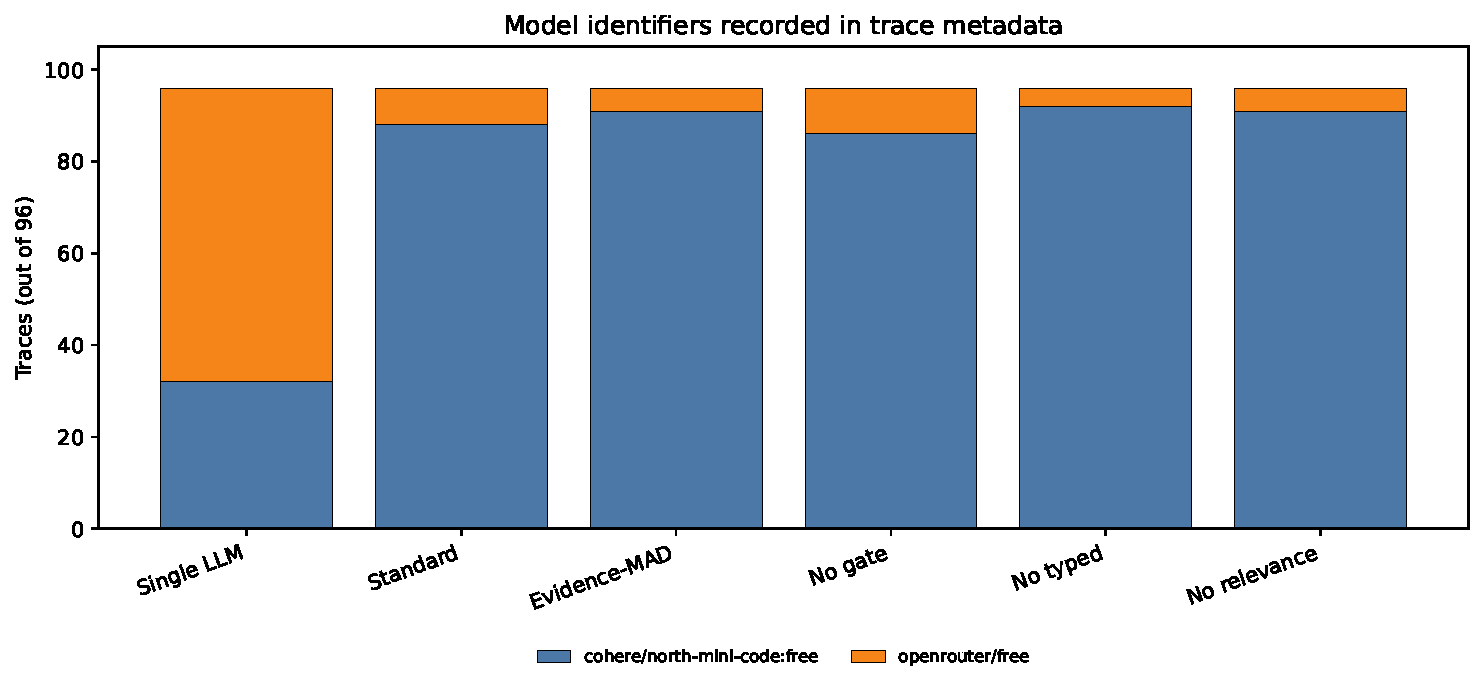
\includegraphics[width=\columnwidth]{model_signature_mix.pdf}
\caption{Recorded OpenCode model identifiers per system. Counts sum to 96 in each bar.}
\label{fig:modelmix}
\end{figure}

\begin{table*}[t]
\centering
\caption{Trace-derived operational results over 96 matched questions. Latency is in seconds; call counts are means per question.}
\label{tab:results}
\small
\begin{tabular}{lrrrrrr}
\toprule
System & Debates & Debate rate & Latency median & Latency $p95$ & Calls OK & Calls failed\\
\midrule
Single LLM & 0/96 & 0.0\% & 16.79 & 26.51 & 1.00 & 0.00\\
Standard MAD & 50/96 & 52.1\% & 54.99 & 211.47 & 1.42 & 0.49\\
Evidence-MAD & 22/96 & 22.9\% & 49.99 & 232.65 & 1.85 & 0.39\\
No Gate & 50/96 & 52.1\% & 49.99 & 200.21 & 1.66 & 0.46\\
No Typed Strategy & 23/96 & 24.0\% & 54.99 & 238.55 & 1.90 & 0.49\\
No Relevance Filter & 18/96 & 18.8\% & 54.96 & 205.42 & 1.57 & 0.39\\
\bottomrule
\end{tabular}
\end{table*}

\section{Discussion}
The traces support a narrow conclusion. In this saved run, the proposed configuration triggered debate less often than Standard MAD, and its median latency was about five seconds lower. Its 95th-percentile latency was about 21 seconds higher. Without gold labels, we cannot tell whether the lower debate rate reflects better selectivity or missed conflicts. Without uniform model metadata, we also cannot attribute the latency differences to the gate or conflict strategy.

The ablation results do not form a clean component-by-component ranking. The no-typed-strategy variant triggered debate on 23 questions, close to Evidence-MAD's 22. The no-relevance-filter variant triggered on 18, fewer than Evidence-MAD. These are trace counts, not evidence that either ablation makes better decisions. Retrieval and normalization can change the claims presented to the gate, and those changes can alter both state and routing.

The many insufficient states deserve attention. Evidence-MAD had 47 insufficient traces, almost half of the matched set. The system may be appropriately withholding a decision when evidence is missing. It may also be failing to retrieve or normalize useful claims. The current data cannot distinguish those cases. Logging the number and quality of retrieved documents, then annotating whether they answer the query, would make the next study more informative.

The traces also show that a completed evaluator record can hide a failed stage. The example trace for the Convention on the Rights of the Child query contains a factual conflict classification, but the proposer call failed and no debate round completed. The record still has a final answer. This example shows why completion, debate activation, completed debate, and answer correctness should be separate measures. The current summary reports call failures, but a future paper should also report the number of debates that reached each stage.

The model identifier mix is a further limitation. The six folders do not use one recorded alias in every trace, and the distribution differs by system. A controlled rerun should pin the same model identifier for all configurations and preserve an immutable run manifest. It should also use a stable retrieval snapshot or record the full retrieved documents so that external search changes do not affect comparisons.

\section{Limitations and Next Evaluation}
This analysis has several limits. First, only 96 of the 100 dataset IDs are shared across all six systems. We use the intersection to keep the plotted sample identical, but this excludes four questions. Second, there are no gold answer labels in the matched trace bundle, so we cannot report answer accuracy or conflict-detection precision and recall. Third, it is a single live run. Search ranking, provider behavior, network conditions, and model availability may change on rerun.

Fourth, system signatures vary by recorded OpenCode model identifier. This makes comparisons observational. Fifth, trace completion does not guarantee successful completion of every model stage. Sixth, the evidence-state labels are system outputs, not independent annotations. The figures therefore describe what the system did, not whether it made the correct decision.

A stronger next study should use the same labelled questions for every system, freeze or archive the retrieved evidence, and use one fixed model configuration. Human annotators should label answer facts, claim-pair relations, and whether a debate is needed. Then the evaluation can report answer accuracy, state confusion matrices, debate precision and recall, unnecessary-debate rate, missed-conflict rate, completed debate rate, calls, cost, and latency. Multiple runs would help show how much live-service variation changes the results. Until that work is done, the present data should not be used to claim that Evidence-MAD improves answer quality.

\section{Conclusion}
Evidence-MAD combines retrieval, claim comparison, and conflict-aware debate. In 96 matched traces, it triggered debate on 22 questions, compared with 50 for Standard MAD. This is a useful description of routing behavior. It is not enough to show that the system is more accurate or that the gate selects the right questions. The traces have no gold answer labels, model identifiers vary across configurations, and some internal calls fail even when the evaluator saves a completed record.

The next step is a controlled, labelled evaluation. The current traces provide a useful starting point: they show where the pipeline stops, how often it debates, and where latency accumulates. They do not yet establish that the proposed method performs better than the alternatives.

\appendices
\section{What the saved traces contain}
Each copied trace includes the question, a trace identifier, routing information, retrieved evidence, normalized claims, evidence decision, debate trigger, conflict metadata where available, debate rounds, final answer, timing and call metrics, and evaluator status. The JSON summary in the parent analysis folder is recalculated from these trace-level fields. The original unmatched files remain in the source results folder and were not silently included in the matched-set plots.

The six system subfolders under \texttt{../traces/} contain the same 96 question IDs. The seven plots in the parent \texttt{plots/} directory and the architecture diagram in \texttt{../architecture/} are supplied in both PNG and PDF format. Model identifier counts are preserved in the JSON summary because this variation is material to any later interpretation.

\section{Practical reading of the figures}
The debate activation plot answers how often each trace records a debate trigger. It does not measure whether debate was warranted. Evidence-state bars show the states recorded by each system; they are not a gold-standard confusion matrix. Latency bars summarize one run and include the long tail of live retrieval and model calls. Call bars include successful and failed model calls across pipeline roles. Retrieval bars report trace metrics for usable agents and extracted claims. The model-signature plot reports configured identifiers found in trace metadata, not a provider-side audit. The architecture figure summarizes intended control flow and is not a trace-derived performance plot.

\bibliographystyle{IEEEtran}
\bibliography{references}
\end{document}
